%! TEX root = ../main.tex
\documentclass[../main.tex]{subfiles}
\begin{document}
\section{Einführung in den 3D-Druck}
\subsection{Historisches}
Der 3D-Druck, auch bekannt als \acrfull{am} oder \it{Rapid Prototyping} ist ein bereits länger bekanntes Forschungsfeld, da bereits im Jahr 1986 das erste Verfahren, SLA (Stereolithographie), von Charles Hull entwickelt wurde. 
Jedoch basierten diese frühen Methoden allesamt auf der Verarbeitung von Polymeren in diversen Formen, zum Beispiel bediente sich SLA einem UV-reaktiven Kunstharz, da Kunststoffe zumeist einfacher zu verarbeiten sind als and Materialgruppen. 
Das wohl bekannteste Verfahren ist FDM (\it{Filament-Deposition-Modelling}), welches im Gegensatz zu SLA mit Spulen an Filament, also \say{Kunststoff-Draht} (meist mit einem Durchmesser von $D=\qty{1.75}{mm}$) arbeitet. 
Dieses Filament besteht aus verschiedenen thermoplastischen Polymeren. Das heißt der Polymer kann aufgeschmolzen werden und wird daraufhin durch eine Düse am \say{Druckbett} aufgetragen Schicht für Schicht.
%Dieser Vorgang ist im Konstrast zu SLA reversibel, da ein Thermoplast immer wieder aufgeschmolzen werden kann.\parencite{BHATIA20231060} Das Kunstharz jedoch wird wenn der Photopolymer ausreagiert hat nie wieder in seinen urspünglichen Zustand zurückführbar sein.\parencite{FACUNDO_1}
Metall-3D-Druck ist in jeder Hinsicht komplexer, da für die Materialverarbeitung von den genutzten Materialien sehr hohe Temperaturen benötigt werden, z.B. für den Edelstahl 316L zwischen \qty{1390}{\celsius} und \qty{1440}{\degreeCelsius} \parencite{610LSTEEL}. Zudem ist auch die Handhabung des Materials kompliziert, da ein Pulver mit einer Körnung von $D_{50}=\SI{30}{\micro\meter}$\parencite[~S.3]{ZAKRZEWSKI2020115} verwendet wird, welches bei Einatmung geringer Mengen bereits zu respiratorischen Problemen führt.
Daher müssen die Druckkammern hermetisch versiegelt sein bei sogenannten Pulverbett-basierenden Verfahren, in welchen das Material frei zugänglich ist in großen Mengen.
Anders dabei sind Schweißraupen-basierende Maschinen, da bei diesen das Pulver nicht frei zugänglich ist, da das Material durch eine Düse ausgestrahlt und aufgeschmolzen wird und nie im rohen Zustand in die Druckkammer kommt.
\begin{figure}[h]
\begin{center}
	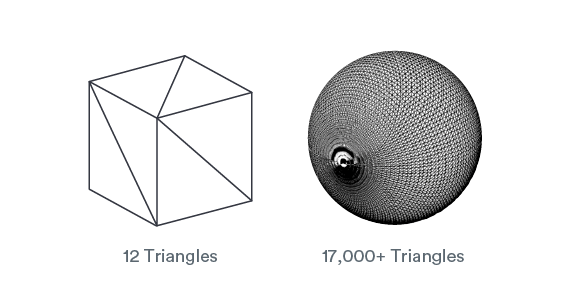
\includegraphics[width=.4\textwidth]{stl_file_1}
	\ccaption{Wireframe eines Würfels und einer Kugel im STL-Datenformat}{\url{https://www.protolabs.com/media/1022944/pl-dt-may-2021_570x308-02.png}}
	\label{img:stl_1}
\end{center}
\end{figure}	

Die Grundlage eines jeden 3D-gedruckten Modells ist meist ein \it{Computer-Assisted-Design-Model} (CAD), welches das gewünschte Teil durch 2D-Zeichnungen darstellt, welche danach zu Körpern extrudiert werden mit verschiedenen Tools. Diese Modelle werden  in \it{Standard-Tesselation-Language} (STL) konvertiert. Dieses Format ist für den \it{Slicer}, ein Programm, welches das Modell für den Drucker konvertiert, verständlich. Ein Slicer (engl. \it{to slice}: schneiden), "schneidet" das Modell in Schichten, welche der Drucker dann auftragen kann. Zusätlich kontrolliert er zumeist die Einstellungen mit welchen der Drucker arbeitet (z.B. Temperatur, Schichtdicke, Geschwindigkeit, o.Ä.). Eine STL-Datei stellt das Modell als eine Punktwolke dar, wobei immer 3 Punkte ein Dreieck, auch bekannt als \it{Facet} oder \it{Face}, bilden. Ein weiterer Aspekt, welcher von STL-Dateien gespeichert wird ist der Normalvektor eines jeden Dreiecks, mit welchem der Slicer berechnen kann, ob es eine "innere" oder "äußere" Wand ist, um eine etwaige Füllung des Teils mit \it{Lattice}-Strukturen, also einem unterstützenden Gerüst, zu ermöglichen ohne das äußere Erscheinungsbild zu beeinträchtigen. Dies ist insofern relevant, da schlecht exportierte STL-Dateien oft fehlerhafte Normalvektoren enthalten und somit beinahe undruckbar sind ohne manuelle Reperatur durch Rückführung in die originale Topologie, welche rechnerisch sehr aufwendig ist und nicht ohne Detailverluste möglich ist.

Das STL-Format ist sehr effizient darin, ebene Oberflächen darzustellen wie Rechtecke, da diese nur aus 2 Dreiecken bestehen. Wenn jedoch eine Krümmung einzurechnen ist, muss wie in Abb. \ref{img:stl_1} zu erkennen ist, diese Krümmung mit Dreiecken angenähert werden. Dieser Vorgang führt eine Ungenauigkeit ein. Diese Problematik kann durch höhere Auflösung des Modells reduziert werden, da die meisten CAD-Suites einen Approximationsgrad angeben lassen (Standardmäßig weit unter \qty{0.1}{\milli\meter}). Die resultierende Dateigröße, welche sich bei schlechter Optimierung schon mit \qty{0.2}{\milli\meter} Approxmiationsgrad bei großen, nicht für den 3D-Druck optimierten Teilen auf \qty{500}{\mega\byte} belaufen kann, sowie auch der stark ansteigende Rechenaufwand sind als Hauptkonsequenz zu beachten. \parencite{ADOBLESTL} 

Als Alternative zum STL-Format steht das STEP-Format, welches Krümmungen mit sogenannten \it{Non-Uniform Rational B-Splines (NURBS)} darstellt.
Diese ermöglichen es, beliebige Kurven und Formen darzustellen. Das Format wird immer beliebter, wobei es noch weit vom Nutzungsgrad der STL-Dateien entfernt ist, da es rechnerisch intensiver ist und von vielen populären Programmen nicht unterstützt wird im Hobby- \& Industriebereich. Die Präzision dieses Formats ist oft hoch gelobt, jedoch in der Praxis aufgrund von schlecht kalibrierten Maschinen sowie auch technischen Limitationen in den meisten Fällen nicht relevant. \parencite{ADOBESTEP}
\end{document}
